% =============================================================
% STRATA (formerly ProcessHeal) — Paper (revised: adds Goals/Objectives + the
%   commercial-BAS-FDD distinction; tightened intro)
% paper-v2.tex     — THIS FILE: adds Method, Verification, Results,
%   Falsified Hypotheses, Errata, Limitations, Conclusion (2026-09-11).
%   Title/abstract realigned to the post-Phase-3 framing. paper.tex is
%   preserved unchanged.
% UREAP 2026, Thompson Rivers University
% Author: Yassh Singh
% Supervisors: Dr. Anthony Aighobahi, Dr. Mridula Sharma
%
% Version history (all in this folder):
%   paper-v1.tex      — first pass, pre-critique
%   paper-draft.tex   — earlier paper-size version
%   paper.tex         — THIS FILE, current working draft
%   literature-review.tex — long survey for the UREAP final report
%
% Compile in Overleaf: Recompile twice. Bibliography in
% references.bib (shared across all .tex files in this folder).
% =============================================================

% =============================================================
% CLAIM -> ARTIFACT TRACEABILITY MAP  (maintained: 2026-09-23)
%
% When an artifact is regenerated, these are the ONLY sentences that
% can move. Check this list before editing prose, and update it when
% you add a claim. Authority order: committed artifact > RESEARCH_LOG
% Part V addendum > ERRATA.md > phase documents (two carry SUPERSEDED
% banners and must never be quoted directly).
%
% Sec.  Claim                                  Artifact
% ----  -------------------------------------  ---------------------------
% Meth  circularity 1.8% vs 5.2%, 81 v 238     benchmark_v2_processheal_v1
%                                              .json + benchmark_v3.json
% Meth  reversal probe .8861/.5526/.9533/      grammar_results.json
%       .9021/.9026
% Meth  retraction 21-117 -> <=2 days;         core/residuals.py (band
%       0.5/0.22/0.02-0.03 degF                constant); phase record
% Res   scorecards 14/14 naive, 13/14          benchmark_v6_*.json +
%       adjudicated, 23/30, 24/29              x11_branch.json
% Res   TTD tails {1x9,2x4} / {1x19,4,11,      benchmark_v6_*.json (naive)
%       (SDAHU adjudicated tail)               + x11_branch.json
%       15,21} / {1x19,3,15,15,37,108}
% Res   FPR 15.6/12.5/4.2 naive; 1.0/5.2/4.2   union_fpr_*.json
%       deployed; genuine-vs-by-construction
%       decomposition (table caption)
% Res   cry-wolf < 0.1%  (adjudicated with     crywolf.json
%       13/14; naive with 14/14)
% Res   windows 137-164 d; conditional recall  benchmark_v6_sdahu.json
%       164/164, 164/164, 139/139, 137/137
% Res   PCA 60v61; 13v13, 23v23, 24v25;        baselines_*.json
%       both-miss 10; PCA strict FPR 1/79,
%       1/96, 1/96
% Res   ablation: 0/73 detected only by       benchmark_v6_*.json
%       model/device; SFPU FP 4/96 -> 1/96    (meaningful_channels) +
%                                              union_fpr_sfpu.json
% Res   matched rules 141=141, 206=206;        matched_rules_*.json
%       MR1 231 SDAHU / 124 PFPU / 0 SFPU;
%       oscillation 349 vs <=2
% Res   attribution 36 correct / 10 none /   alarm_attribution.json
%       0 wrong of 46; 14 no stratum; 1 indet. (naive 61-detection universe)
% Res   onboarding 45 mappings + 35 rules,     configs/ONBOARDING_LOG.md
%       ~1.5 h (reconstructed from commits)
% Fals  192 v 135 (+ min-robust 22-26)         matched_rules_sfpu.json
% Fals  X11: 0 flags on 148 window days        x11_branch.json
% Fals  contamination 164/164 -> 0/164;        x8_contamination.json
%       visibility 5/5,13/13,27/27 vs 0/27
% Fals  sampling 28/64/64; FOUR falsifiers     x7_downsample.json
% Ver   >100 tests (floor test); SDAHU byte-repro tests/ + REPRODUCING.md
% Erra  E1-E5                                  ERRATA.md + week0_audit.json
%
% Fals  discovery-predicts-transfer: Q .978/.455/0, discovery_predicts_transfer.json
%       firings 124,0,1 / 0,0,0; rho -.693,       (+ _q.json; prereg + amendment
%       exact p .200; never had power (cluster   in docs/plans/2026-09-23-*,
%       min p .167); F2 void; no conclusion       amendments 1-3)
% Erra  E5 damper floor 0.000 vs 0.100             ERRATA.md E5
% Erra  E3 leakage: healthy-only threshold, 365/365  e3_leakage.json
%       and 0/7150 misclassified, acc 1.0 both cols
% PENDING (now a Limitations subsection, no numbers):
%   open-fdd G36 comparison - artifacts VOID, see
%   strata/docs/plans/NEXT-openfdd-baseline-repair.md
% =============================================================

\documentclass[11pt,letterpaper]{article}

\usepackage[margin=1in]{geometry}
\usepackage{microtype}
\usepackage[hidelinks]{hyperref}
\usepackage{cite}
\usepackage{times}
\usepackage{graphicx}
\usepackage{array}

\title{STRATA: Seven Adverse Results and a Detector\\ \large HVAC fault detection under a falsification protocol}
\author{Yassh Singh \\
\small Supervisors: Dr.\ Anthony Aighobahi, Dr.\ Mridula Sharma \\
\small Thompson Rivers University --- UREAP 2026}
\date{September 2026}

\begin{document}
\maketitle

\begin{abstract}
\noindent
We report STRATA, a fault-detection framework for building HVAC systems, together with the falsification protocol under which it was built: hypotheses pre-registered with the observation that would refute them, results recomputed independently from raw data before they are quoted, and automated tests that pin published numbers, fired falsifiers, and disclosure obligations. The protocol refuted the project's founding hypothesis. Process models discovered from fault-free operation were expected to detect faults; a one-line hand-written rule out-covered them, and an ablation over all 73 seeded scenarios finds no fault detected only by the discovered models --- removing them changes no scorecard and lowers one system's false-alarm rate. A sealed, pre-registered test of the fallback claim, that the models predict where a rule transfers between buildings, never had attainable power, as its third amendment records; it is reported as a protocol failure, not a result. What survives is a detector of eight calibrated, physically interpretable channels that on three public LBNL benchmarks --- two never previously benchmarked --- detects 13 of 14, 23 of 30 and 24 of 29 seeded faults at a median of one day, with a stated false-alarm budget of 1.0--5.2\% of fault-free days (15.6\% on the air handler with every channel counted), naming the correct terminal unit in 36 of the 46 detections with determinable ground truth on the two systems with a device stratum, none in 10, and a wrong one in none. A principal-component baseline ties it on detection and has fewer false alarms on the two terminal-unit systems, with all intervals overlapping; it cannot name the device. The evaluation also produced five previously unreported, machine-verified errata in the benchmark datasets. Every number regenerates from the public repository.
\end{abstract}

\section{Introduction}

Buildings account for approximately 34\% of global energy-related carbon dioxide emissions, and HVAC systems carry the dominant share within that total \cite{bi2024aihvacreview}. The fraction of HVAC energy wasted by undetected faults has consistently been estimated at 15--30\% across recent reviews \cite{bi2024aihvacreview,pritoni2022faultcorrection}, but until late 2023 these numbers rested on relatively small studies. The first large-scale empirical characterisation appeared when Crowe and colleagues analysed multi-year fault-detection output across more than 60{,}000 pieces of HVAC equipment in 317 commercial buildings \cite{crowe2023faultprevalence}. Their study reports an average of 245 faults per building per month and finds 40\% of all air handling units in a faulted state on any given day. The most common AHU fault in their dataset, a supply-air-temperature setpoint that is never reset, was observed on 55\% of the AHUs surveyed. These buildings were not unmonitored; many run modern building automation systems with alarms and fault-detection features, yet the faults persisted, which points to a gap in the kind of fault these tools can see rather than in their deployment.

The nature of that gap is specific. Of the ten most common AHU faults catalogued by Crowe and colleagues, seven are behaviour-based rather than condition-based: incorrect schedules, unreleased manual overrides, missed setpoint resets, and broken economiser sequences manifest as deviations in the temporal ordering of system states rather than as isolated component failures. A threshold alarm fires when a single variable leaves its acceptable band, and a pre-programmed rule fires when a named fault pattern is matched, but neither mechanism detects a control sequence that executes its steps in the wrong order or skips a step entirely unless a rule was written for that specific sequence in advance --- which is possible, and has been done for logic faults \cite{gunay2022logicfaults}, but only for the sequences someone anticipated. The structural argument that follows is straightforward: detection methods that model the sequence in which a building moves between operating states have a natural advantage on the fault classes that dominate the empirical landscape.

The dominant research methodology for HVAC fault detection does not model that sequence either. Machine learning has been surveyed across 211 AI-based HVAC FDD studies published between 2013 and 2023 \cite{bi2024aihvacreview}, with reported accuracies on the standard benchmarks saturating at 97--99\% across hybrid random-forest pipelines on RP-1312 data \cite{tun2021hybridrfsvm} and convolutional-and-LSTM hybrids on real-building data \cite{prince2025improved1dcnnlstm}. The most recent work has shifted toward interpretability, but in a specific way: a deep model is paired with a post-hoc explanation method such as layer-wise relevance propagation or attention attribution \cite{deng2024afgcn,wang2025xmhac}. The resulting explanation is at the level of input features rather than at the level of the control sequences the building was supposed to follow. A facility manager told that sensor $X$ had high relevance for a prediction knows that something is unusual about that signal, but is not told how the building was supposed to be behaving instead.

A second problem concerns reproducibility. A recent audit of 65 primary machine-learning HVAC fault detection studies, circulated as a preprint, found two that shared code links, one of them broken, and that 72\% do not specify whether their dataset is public, proprietary, or commercial \cite{mukhtar2025reproducibility}. The field has plateaued on accuracy, a metric that does not measure what an operator needs, with little of the existing work independently verifiable, and with the dominant explanation style answering a question (which signal mattered) different from the one operators ask (what should the system have been doing).

The opportunity is to change the model class. Process mining is a methodology in which a discrete event log derived from system observations is used to discover a Petri-net model of expected behaviour, with conformance checking against that model producing an alignment-based deviation signal that carries formal fitness and precision semantics \cite{vanderaalst2016processmining}. We apply this approach to HVAC fault detection, treating sensor-derived events as the input log and ASHRAE Guideline 36 control sequences as the conceptual reference. Our initial hypothesis was that the discovered Petri net would serve as both the expected-behaviour model and the detector. That hypothesis was pre-registered, tested, and refuted: a single hand-written rule out-covered the unit-stratum model channel on the scenario where that channel was strongest. What survived the refutation is narrower. The discovered models served as design-time scaffolding: they surfaced candidate invariants that a domain expert then wrote as rules, and once those rules existed the models contributed no detection of their own. Whether the models can predict, in advance, where such a rule will hold on another building is a further claim this paper set out to test and could not (Section~\ref{sec:falsified}). Detection is done by calibrated, physically interpretable channels against a measured noise floor. Section~\ref{sec:falsified} reports the refutation in full.

Four contributions follow, and the order is deliberate. First, the evaluation protocol --- pre-registration, honoured falsifiers, adversarial recomputation, tests that pin disclosures, and full artefact regeneration --- in a subfield where an audit of sixty-five primary studies found two that shared code links, one of them broken \cite{mukhtar2025reproducibility}. Second, one pre-registered negative result about process mining on this domain --- discovered models detect no fault that calibrated channels miss --- and one pre-registered test of whether they predict where a hand-written rule transfers, which never had attainable power, as its third amendment records, and which is reported as a protocol failure rather than as a result in either direction. A precedent for the shape of this result exists in another cyber-physical domain: Zhong and Lisitsa report, in a preprint, that na\"{i}ve process mining on network event logs was ineffective for intrusion detection \cite{zhong2022pmids}. This remains, to our knowledge, the first application of event-log process mining to building HVAC fault detection, corroborated by the one systematic review of process mining on sensor data whose scope could have captured such work \cite{brzychczy2025pmsensorreview}; the claim is that the application was made and tested, not that it succeeded. Third, a detector that reports at a stated false-alarm budget rather than at accuracy alone, evaluated on three public benchmark systems, two of which had not previously been benchmarked, with one alarm shown verbatim. Fourth, five machine-verified errata in the benchmark datasets. Deployment on an operating building remains the intended next phase.

\section{Research Aim and Objectives}
\label{sec:aims}

The aim of this research is to establish process mining as an interpretable and generalisable approach to fault detection and diagnosis in building HVAC systems. The work reported here is validated on public benchmark data; deployment on an operating building is the intended next phase rather than a result of this paper. Six objectives define the current scope:

\begin{enumerate}
\item \textbf{Abstract events from sensor data.} Convert continuous HVAC sensor streams into discrete event logs using control-sequence rules grounded in ASHRAE Guideline 36, with fault-signature events held out of model discovery so that the models cannot re-detect the rules that produced them.
\item \textbf{Discover models and locate invariants.} Learn Petri-net models of expected control behaviour from fault-free data at device, unit and cross-system granularity, and establish what those models contribute. This objective is reported in the form its own falsification required: the models served as design-time scaffolding that surfaced candidate invariants, and contribute no detections once the corresponding rules exist (Section~\ref{sec:falsified}).
\item \textbf{Detect against a measured noise floor.} Calibrate interpretable channels on fault-free data alone and require every alarm to exceed that channel's own measured noise, so that detection is reported with a stated false-positive budget rather than with accuracy alone.
\item \textbf{Benchmark against known answers.} Evaluate on the LBNL benchmark family --- a single-duct air-handling unit and two fan-powered-unit configurations --- against documented ground-truth faults, and compare with a machine-learning baseline on identical scenario universes and with a third-party implementation of the ASHRAE Guideline 36 rule battery representing current commercial practice.
\item \textbf{Make every claim checkable.} Pre-register each hypothesis with the condition that would refute it, subject every result to adversarial recomputation before it is quoted, and guard published values, fired falsifiers and disclosure obligations with automated tests.
\item \textbf{Release the work openly.} Publish the pipeline and its building configurations as open-source software, evaluated on public data with a documented path from a fresh clone to regenerated artefacts, addressing the reproducibility gap identified in the literature.
\end{enumerate}

\noindent Objectives one to three constitute the method and are reported in Sections~\ref{sec:method} and~\ref{sec:results}; objective four is reported in Section~\ref{sec:results}, with the Guideline 36 comparison still in progress (Section~\ref{sec:baseline}); objectives five and six run throughout and are described in Section~\ref{sec:protocol}.

Two goals lie outside this scope and are stated as future work rather than quietly dropped. The first is a hybrid extension combining process-mining features with machine-learning classifiers, deferred for the reason given in Section~\ref{sec:limitations}. The second is deployment on an operating building --- live trend data from Thompson Rivers University's Campus Activity Centre, delivering a ranked diagnostic report that complements the rule-based detection already present in its automation system. The contamination result of Section~\ref{sec:falsified} is the principal technical obstacle to that deployment and is why it is not attempted here.

\section{Related Work}
\label{sec:related}

\subsection{Machine learning for HVAC fault detection, and the move from accuracy to interpretability}

The machine-learning era of HVAC fault detection is well documented. Bi and colleagues survey 211 AI-based HVAC FDD studies published between 2013 and 2023, organising them into traditional machine-learning, deep-learning, hybrid AI, and physical-model branches \cite{bi2024aihvacreview}. Reported accuracies on the standard benchmark datasets have effectively saturated. Tun and colleagues reached 98\% accuracy across thirteen fault types using a hybrid random-forest and support-vector-machine pipeline on RP-1312 AHU data \cite{tun2021hybridrfsvm}. Prince, Yoon, and Kumar reached 97\% accuracy on data from three real buildings using a thirteen-layer one-dimensional convolutional-and-LSTM hybrid that remains robust to Gaussian noise and to 10\% missing values \cite{prince2025improved1dcnnlstm}. The authors of that paper close by explicitly identifying interpretability as the problem they did not solve, proposing grafting SHAP or LIME as future work.

The most directly relevant interpretable benchmark for the LBNL SDAHU subset is Deng and colleagues' adaptive fusion graph convolutional network. The model reaches 88.09\% accuracy at 500 labelled samples and 75.15\% at only seven samples, with per-node sensor importance as the explanation mechanism \cite{deng2024afgcn}. Subsequent work in the same vein pairs multi-head attention with parallel dilated convolutions and applies layer-wise relevance propagation for explanation on chiller fault data, reaching an F1 score of 0.9841 across 27 operating conditions \cite{wang2025xmhac}. The pattern across this body of work is consistent: a deep black-box network is the model, a post-hoc analysis layer provides the explanation, and the explanation is framed at the level of input features rather than control flow. The architectural opportunity is for a method whose model is its explanation.

\subsection{Unsupervised methods and cross-building deployment}

Real buildings rarely come with ground-truth fault labels, and the strongest recent work on unlabelled data uses self-supervised or autoencoder methods. Abdollah and colleagues pretrained a Transformer encoder via masked-token reconstruction on unlabelled HVAC time-series from a heat-pump building at the Polytechnic University of Milan, then used Peak-Over-Threshold detection on reconstruction error to flag a real two-month monitoring fault between October and December \cite{abdollah2024transformerssl}. The most directly relevant precedent for a Canadian-university real-BAS deployment is El Mokhtari and McArthur's autoencoder-based work at Toronto Metropolitan University, which distinguishes equipment-level from system-level faults across five fan coil units and demonstrates cross-unit transfer learning \cite{elmokhtari2024aebas}. These methods share a common limitation. Each produces a learned latent embedding whose deviation signal is a scalar anomaly score, not a process-level explanation.

The cross-building generalisation problem is the binding constraint that prevents most existing HVAC FDD work from being deployed in the field. The established response is domain adaptation, which transfers learned network weights: Zhu and colleagues migrate fault detection between two different building chillers \cite{zhu2021chillertransfer}, and Ghalamsiah and colleagues apply a contrastive adaptation network to ASHRAE-1312 simulation as a labelled source and real AHU measurements as an unlabelled target \cite{ghalamsiah2025canhvac}. What STRATA transfers between buildings is a configuration file naming sensors and rules, not a set of learned weights; transferring it is therefore a different operation from the weight transfer the literature above studies, and Section~\ref{sec:falsified} reports that the discovered models themselves did not transfer.

\subsection{Process mining: foundations, adjacent successes, and the empty quadrant in building energy}

Process mining was formalised by van der Aalst as a methodology for discovering process models from event logs, checking observed behaviour for conformance, and enhancing the resulting models with additional perspectives \cite{vanderaalst2016processmining}. Conformance checking was used directly as a trace-level anomaly detector on event logs \cite{bezerra2013anomalytraces,rozinat2008conformance}; the line subsequently moved to neural sequence models that outperform conformance-based baselines on standard log corpora \cite{nolle2022binet}. The conformance channels used here are the nearest descendant of the former, and the ablation reported in Section~\ref{sec:results} --- no fault detected only by them --- is consistent with the motivation for the latter. The methodology has also been applied across cyber-physical and sensor-driven domains adjacent to building energy. Vitale and colleagues applied a full process-mining pipeline to fault diagnosis on the RoAD robotic-arm dataset, reaching an F1 score of up to 98.925\% with a conformance-checking time as low as 0.020 seconds \cite{vitale2025roadcps}. The same group then demonstrated that combining process-mining-derived alignment features with downstream dimensionality reduction substantially outperforms pure conformance checking across four cross-domain datasets, with F1 improvements ranging from 30 to 70 points \cite{vitale2025kbsfeatures}. Husom and colleagues' UDAVA pipeline extended this hybrid pattern to industrial Internet-of-Things sensor validation \cite{husom2026udava}. Methodologically the closest analogue to building HVAC is Moradbeikie and colleagues' work on pasteurisation, where continuous multivariate sensor signals are abstracted into discrete activity sequences via hidden Markov models and conformance is checked against HACCP critical control points \cite{moradbeikie2025pasteurization}. Pasteurisation, like HVAC operation, is a continuous-flow process governed by an explicit regulatory standard; the analogy between HACCP critical control points and ASHRAE Guideline 36 control sequences is suggestive. It is not a direct port: pasteurisation has a single physical flow and a case notion given by the batch, whereas HVAC operation has no natural case boundary, concurrent devices at several granularities, and an alphabet in which some events already encode fault suspicion --- both the case notion used here (the calendar day) and the partition of the event alphabet had to be constructed. The technical barrier common to all these applications is event abstraction, the conversion of continuous sensor time-series into discrete activity sequences, which was formalised in the methodology paper by Janssen and colleagues \cite{janssen2021sensoreventlog}.

Despite these adjacent successes, building HVAC remains an empty quadrant in the literature. The novelty claim rests principally on one review and is corroborated by three others whose scope or period would not necessarily have captured such work. Bi and colleagues' survey of 211 AI-based HVAC FDD studies contains no process-mining entries in any leaf of its method taxonomy \cite{bi2024aihvacreview}. Akhramovich and colleagues' review of 47 process-mining studies in Industry 4.0 covers manufacturing, internal logistics, mining, alarm management, supply-chain logistics, and product lifecycle management; building applications do not appear \cite{akhramovich2024pmindustry40}. Where process mining has reached the built environment at all it is for construction and facility-management workflows \cite{martinezlagunas2024constructionpm}, with cases as projects and activities as human tasks; the operational control flow of a building's mechanical systems is not addressed. Brzychczy and colleagues' more recent review of 36 process-mining studies on sensor data documents the same absence at finer granularity: fourteen industrial applications, eleven smart-home applications (all motion-sensor occupant-activity recognition), seven healthcare applications, two smart-office applications, two smart-product applications, and one other, with no building HVAC \cite{brzychczy2025pmsensorreview}. The Lawrence Berkeley National Laboratory team's canonical FDD-methods taxonomy from 2017 organises automated fault-detection methods into quantitative model-based, qualitative model-based, and process-history-based categories, and process mining is not present at any leaf \cite{granderson2017fddtoolsurvey}. The absence is consistent across all four, and our own exact-phrase searches of the OpenAlex corpus for process mining or conformance checking in conjunction with HVAC, building automation, air handling, or chillers return no work; nor did the ICPM 2025 programme, the most recent at the time of writing, contain any. No published work, to our knowledge, applies event-log process mining to building HVAC fault detection.

\subsection{Rule-based fault detection in practice, and what process mining adds}

Fault detection is not absent from real buildings; it is simply rule-based. The most widely deployed form is the fault-detection capability embedded in commercial building automation systems. Modern platforms ship libraries of pre-programmed fault rules: the Automated Logic WebCTRL system used at the deployment building of the present study, for example, includes a standard library that matches over one hundred named faults in common HVAC equipment.\footnote{Automated Logic, \emph{Fault Detection and Diagnostics}, \url{https://www.automatedlogic.com/en/products/webctrl-building-automation-system/integration/fdd-reporting-and-dashboards/}.} The characterisation survey of fourteen commercial FDD tools by Granderson and colleagues confirms that this rule-based and threshold-based style is the norm across the commercial landscape \cite{granderson2017fddtoolsurvey}, and Guideline 36's fault conditions have themselves been used as the reference against which learned diagnostic models are built \cite{pradhan2021dbng36}. The strength of a rule library is that it works immediately on connection and requires no baseline data; its structural limitation is that it can only detect the fault patterns that were coded into it in advance, and so it misses novel failure modes and the gradual, multi-variable, sequence-level deviations that no rule author anticipated.

The same rule-based philosophy characterises the most directly comparable research programme, the Lawrence Berkeley National Laboratory team's automated fault-correction line. Pritoni and colleagues field-tested seven hand-coded correction algorithms across 225 distinct equipment items in four buildings on three building-automation-system platforms, targeting common control problems such as incorrectly programmed schedules, unreleased manual overrides, and missed setpoint resets \cite{pritoni2022faultcorrection}. Each algorithm is a pre-encoded rule matched against BAS data and applied through a two-way BACnet writeback to the building's control system. Both the commercial libraries and the LBNL correction algorithms share the assumption that the faults of interest can be enumerated and encoded ahead of time.

STRATA makes the opposite assumption and is therefore complementary to both. Rather than matching observed data against a fixed catalogue of known faults, it learns from the building's own fault-free operating data where that building's behaviour is invariant, and calibrates detection channels to hold those invariants. Conformance alignment against the discovered models is one such channel rather than the whole detector --- a distinction our own results forced on us (Section~\ref{sec:falsified}) --- and it contributes the property a rule library cannot supply unaided: during development the invariants were surfaced by discovery rather than enumerated in advance, which is how several of the rules now deployed came to be written. Every channel carries a measured false-alarm budget, which is what makes the resulting alarms answerable rather than merely numerous. A practical consequence is that STRATA can run on the same trend data a commercial system such as WebCTRL already records, addressing the behaviour-based and sequence-level faults that fall outside the rule library and below the alarm threshold, while the rule library continues to handle the well-understood patterns it was built for. In principle the conformance traces STRATA produces could serve as input to the LBNL correction algorithms, extending automated correction beyond the patterns pre-encoded by hand. The LBNL FDD dataset family \cite{granderson2020lbnlfdddata} provides the labelled simulation testbed that supports this complementary positioning.

One adjacent body of work must be distinguished as a class, because its vocabulary is similar. Hand-designed Petri nets have modelled HVAC and building systems for two decades --- for hybrid system modelling \cite{villani2004hybridpetri}, for building-automation monitoring \cite{gomes2007petribas}, and for chiller fault diagnosis \cite{xu2015chillerpetri} --- and in every case the net is authored by an engineer rather than discovered from a log. The most recent example is control: Deabes, Bouazza, and Algthami designed a fuzzy Petri-net controller for HVAC temperature regulation, hand-engineering both the Petri-net structure and the fuzzy rules and using the model as a forward control device for an air-conditioning compressor \cite{deabes2023fuzzyptn}. None of this work contains an event log, a process-discovery algorithm, or alignment-based conformance checking; the diagnosis variant matches observations against a net an expert drew. The present work does the methodological opposite: a Petri net is discovered from a real event log of HVAC operation, then used as a reference against which alignment-based conformance checking diagnoses operational deviations. Hand-designed Petri-net controllers and data-discovered Petri-net diagnostic models are two distinct uses of the Petri-net formalism, and they should not be conflated.


\section{Method}
\label{sec:method}

STRATA (Figure~\ref{fig:framework}; code and artefacts at \url{https://github.com/iyassh/strata}) consumes one fault-free year of ordinary building-management-system trend data together with a single configuration file naming the building's sensors and control rules. That configuration file is the only site-specific artefact: no code change was required to onboard any system reported here.

\begin{figure}[t]
\centering
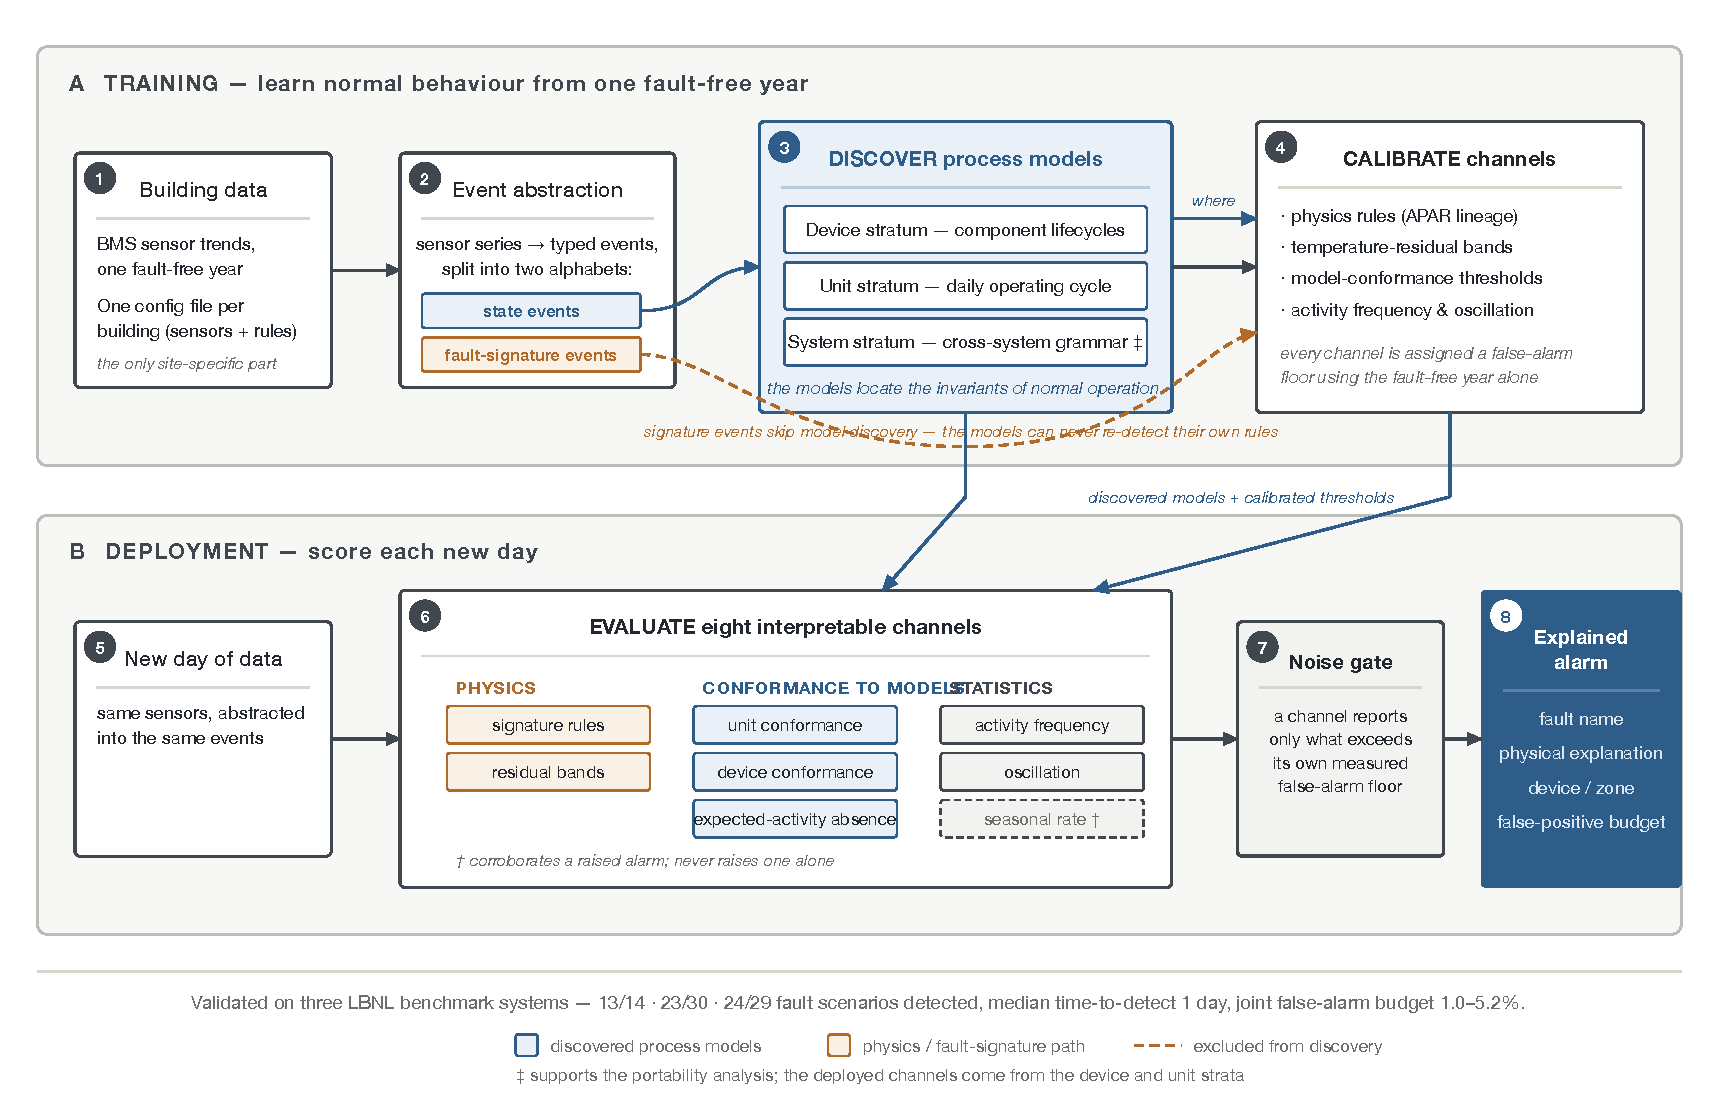
\includegraphics[width=\textwidth]{figures/strata_framework_v2.pdf}
\caption{The framework. Training (top): one fault-free year and one configuration file; events are split into state and fault-signature alphabets, models are discovered from state events only, and every channel is calibrated to its own noise floor. Deployment (bottom): each day is scored by every channel, only what clears a channel's floor may report, and what survives reaches the operator with a name, the evidence, and that channel's stated false-alarm budget.}
\label{fig:framework}
\end{figure}

\subsection{Event abstraction and the alphabet wall}

Continuous sensor streams are converted into a discrete event log using control-sequence rules grounded in ASHRAE Guideline 36, following the abstraction methodology of Janssen and colleagues \cite{janssen2021sensoreventlog} and the taxonomy of event abstraction in van Zelst and colleagues \cite{vanzelst2021eventabstraction}. The events are then partitioned into two alphabets that are never mixed. \emph{State events} are neutral facts about operation and are the only events admitted to model discovery. \emph{Fault-signature events} already encode engineering suspicion and are withheld from discovery entirely.

The partition --- the alphabet wall --- exists because of circularity, the process-mining form of the data-leakage problem \cite{weytjens2022dataleakage}: a model discovered over an alphabet that already names faults will later ``detect'' those faults by recognising the project's own rules. Comparing this pipeline's partitioned artefact against the committed artefact of its pre-partition prototype on the single-duct system --- same threshold, same 248-day train and 87-day holdout split, same 4{,}540 fault days, and an identical rules-channel output of 3{,}134 true positives, but not the same code version --- the model channel's apparent recall rises from 1.8\% to 5.2\% (81 days against 238) without the partition. The two artefacts agree on every combined-detector number (3{,}152 true positives, 5 false positives), so the partition changed the deployed detector's output by zero days: every model-channel detection the leak supplied was already caught by the rules channel. A controlled same-code re-run is future work; the deployed scorecard, two code generations later, gives the same reading (86 model-channel days of 4{,}891 evaluable fault days, 1.76\%). That 3.5-percentage-point difference (5.24\% against 1.78\%) is a measured bound on model self-confirmation, and the separation is now enforced by a tested invariant: injecting signature events into a log cannot change a day's fitness. The process-mining literature warns about this trap in the abstract; we are not aware of a prior quantification of it on sensor-derived logs.

\subsection{Discovery at three strata}

Petri nets are discovered from the state-event log with the inductive miner \cite{leemans2013inductiveminer,leemans2014inductiveminerinfrequent}, as implemented in pm4py \cite{berti2023pm4py}, at three granularities: the device stratum models an individual actuator's lifecycle, the unit stratum models the air handler's daily operating cycle, and a cross-system grammar supports the transfer analysis of Section~\ref{sec:falsified}.

Whether a discovered net encodes temporal order at all --- rather than merely a set of permitted activities --- is the question precision metrics address \cite{munozgama2010precision,buijs2012quality,tax2018imprecisions}, and the imprecision of precision on logs without negative examples \cite{vandenbroucke2014negativeevents} is why we use a direct probe instead. The \emph{reversal probe} is that direct check: every trace is reversed and re-scored, and the fitness drop is reported as a single number. The three models separate cleanly. The single-duct net falls from 0.8861 to 0.5526 under reversal, confirming genuine order sensitivity. The series fan-powered net scores identically to four decimal places (0.9533 against 0.9533) and the parallel net shifts by 0.0005 (0.9021 against 0.9026), showing that neither carries meaningful ordering information in its fitness. The probe is cheap, decisive and reusable, and it converted an informal claim about alphabet complexity into a measured fact.

\subsection{Calibrated channels and the noise gate}

Eight channels evaluate each day independently: (1) \emph{rules}, physics rules descended from the NIST APAR lineage that name direct contradictions between measurements; (2) \emph{residual}, temperature-residual bands encoding relationships that must hold under known operating modes --- with the cooling coil inactive, supply-air minus mixed-air temperature should equal the supply-fan heat rise, so a biased sensor appears as a persistent offset; (3) \emph{model conformance} and (4) \emph{device conformance}, alignment cost \cite{vanderaalst2012replaying,carmona2018conformancechecking} against the discovered unit and device models respectively --- these two are the process-mining channels; (5) \emph{absence}, a scheduled activity that did not occur; (6) \emph{frequency} and (7) \emph{oscillation}, statistical bands on activity counts and reversals; and (8) a seasonal \emph{rate} channel that corroborates but may not raise an alarm alone, for reasons disclosed in Section~\ref{sec:limitations}.

Calibration uses the fault-free year only, at a false-positive quantile of 0.01 against a calendar-stratified holdout of the last eight days of each month. No threshold may see fault data. Every rule additionally requires a positive control, because silence is not competence: a position-based leak rule proved structurally deaf on the fan-powered units, where the seeded leak passes water through a valve whose position reads closed honestly, and was replaced by a waterside flow rule.

A channel may then report only what exceeds its own measured noise floor, tested as a binomial against that channel's own holdout rate at $p<10^{-3}$. Detection thresholds are additionally floored at sensor physics: an early result on the series unit was retracted to at most two detection-days when a 0.5\,$^\circ$F sensor-precision floor revealed that the ``detections'' had exceeded a 0.22\,$^\circ$F band by 0.02 to 0.03\,$^\circ$F.

What survives the gate reaches the operator with the implicated device or zone, the evidence that triggered it, and the channel's own false-alarm budget. Figure~\ref{lst:alarm}, in Section~\ref{sec:results}, is one such alarm from the first day of a seeded fault, every value read from the committed artefacts and the raw data.


\section{Verification as a First-Class Result}
\label{sec:protocol}

An audit of sixty-five primary machine-learning HVAC fault-detection studies found two that shared code links, one of them broken, and 72\% that did not state whether their data was public, proprietary or commercial \cite{mukhtar2025reproducibility}. A field in that condition does not need another accuracy figure; it needs results that can be checked. We therefore treated verification as a deliverable rather than as hygiene, and this section describes the machinery in enough detail to be adopted. The refutations it produced are reported in Section~\ref{sec:falsified}.

\subsection{Pre-registration and honoured falsifiers}

Every experiment is pre-registered: the hypothesis, and the specific observation that would refute it, are committed to version control before the experiment runs, in the spirit of the hypothesis-testing discipline recently urged for process-mining research \cite{pitsch2025hypothesistesting}. A falsifier that fires is treated as a finding and published, not as a setback to be absorbed by rewriting the hypothesis. Seven results went against the project --- three refuted hypotheses, three withdrawn claims, and one pre-registered test that never had attainable power --- several of them results the project would have preferred to keep. Section~\ref{sec:falsified} reports each with the claim it killed and what survived.

The discipline exists because of a failure mode we observed in ourselves. One phase report, drafted the same day as its discovery, contained six distinct overclaims; all six were caught by audit within hours. Positive results attract inflated framing faster than negative ones attract scrutiny, and a falsifier is only protective if it is written down before the result it would kill is known.

\subsection{Gates before science}

Before any detection result is computed, a battery of gates runs against the raw data. It verifies file integrity by MD5, checks that timestamps increase monotonically, confirms that each file's calendar is internally consistent, checks the raw files for calendar rotation, checks coverage of the Brick semantic model, and hashes each derived event log so that duplicate scenarios cannot masquerade as independent evidence. A separate healthy-silence gate is run per configuration, confirming that the rule set is silent on the fault-free year before it is permitted to score anything.

These gates were not designed in advance; each was added after a dataset defect got past the previous set. Two of the five errata in Section~\ref{sec:errata} were found by this battery rather than by inspection --- E1 and E2 by the integrity hash. E4 was found by an early-phase audit; the calendar-rotation gate that now evidences it on the raw files was built four phases later, because the monotonicity check runs on converted files that conversion has already sorted and so could never have caught it. E3 was found by auditing our own baseline and E5 by a later hostile audit, which is the argument for running it: the defects are not visible in summary statistics, and every one of them would have inflated a published result.

\subsection{Three levels of regression}

Guards run at three levels. At the first, more than a hundred automated tests execute on every commit through continuous integration; the data-dependent tests skip rather than error when the datasets are absent, so the suite is meaningful on a bare clone. At the second, a regeneration gate re-derives committed artefacts from source and diffs each against its stored copy, reporting per artefact either an identical verdict or a named set of changed values. A changed verdict is a defect or a documented decision, never a silent update. At the third, every newly validated dataset is frozen permanently into the suite as a fixture, so that the examination the method must pass only ever grows.

The single-duct system is the byte-reproducibility standard: re-running its benchmark must reproduce the committed artefact byte-identically, and that requirement is enforced after every change. The fan-powered-unit artefacts are regenerated and diffed but carry no equivalent standing guarantee.

\subsection{Tests that pin refutations and disclosures}

The unusual property of the suite is what it guards. Alongside conventional unit tests of the event, residual, frequency and grammar logic, it pins three things that are not ordinarily thought of as testable.

It pins published values, so that a change which would alter a number quoted in a paper fails the build rather than propagating silently. It pins \emph{fired falsifiers}: the sampling-rate experiment's finding \emph{is} its four refutations, and a regeneration that loses them is treated as a regression exactly as a lost feature would be. And it pins \emph{disclosure obligations}. One test asserts that the artefact continues to declare which channels' false-positive rows are calibration targets rather than out-of-sample measurements --- the caveat reproduced in Section~\ref{sec:limitations}. Another asserts that the post-selection defence ships alongside the result it defends. A third recomputes the cry-wolf ratio from the benchmark and union artefacts rather than reading the stored value, so that an internally consistent but wrong number cannot survive; a fourth recomputes sensor coverage from the configuration files for the same reason.

Continuous integration has been used to guard that a published result regenerates \cite{jimenez2017popper}. What we have not found reported is CI that guards that a published \emph{caveat} survives: a regeneration that drops a disclosure fails the build exactly as a lost feature would. Its justification is that caveats decay faster than code: a sentence in a document can be dropped in a rewrite without anything failing, whereas a test that enforces the sentence cannot.

\subsection{Adversarial audit}

By \emph{adversarial audit} we mean an independent recomputation of a claimed quantity from raw data by someone briefed to find it wrong --- in this project, AI coding agents given that brief and, for the sealed test of Section~\ref{sec:falsified}, denied access to the answer key --- not the red-teaming of a model that the phrase denotes elsewhere. Before any number is quoted, it is attacked in this sense. An audit is briefed adversarially --- to assume the result is wrong and to find the ways its authors have flattered themselves --- and independently recomputes the quantity from raw data rather than re-running the pipeline that produced it, so that a defect in the pipeline cannot confirm itself. Independence of implementation is the point: on more than one occasion the recomputation agreed with the artefact and disagreed with the prose written about it.

The method's value is measurable in what it caught. It found that a baseline was detecting file provenance rather than faults. It found that one of the fourteen single-duct detections was an artefact of the dataset --- the fault-free file was simulated on a different configuration branch than every fault file, and the detector was noticing the branch, not the fault --- so the score is reported as 14/14 naive and 13/14 adjudicated. It found that a day-level significance test adopted in Phase 4 rested on an impossible null, the discordant cell it tested being zero by construction; the test was retracted, the significance it had awarded was withdrawn, and a binomial against each channel's own noise replaced it. It found detections below sensor precision, an evidence sentence falsified by its own recomputation, and, most recently, a completed comparison against commercial practice invalid for three independent reasons (Section~\ref{sec:baseline}). None of these would have been caught by a test suite, because in each case the code was doing what it was written to do.

\subsection{The lesson ledger, and why documentation decays}

Thirty-two numbered lessons record each failure with the standing rule it produced. The ledger is itself a result, because a pattern emerges from it that we did not anticipate.

The first pattern is recurrence: the same lesson reappeared in different clothing. A rule requiring day universes to be derived from the raw calendar rather than from the event log was recorded, documented, and then violated again two phases later. The conclusion drawn, and now standing policy, is that \textbf{a lesson is not closed until a helper or a test mechanically enforces it} --- documentation alone decays. Several of the tests described above exist for precisely that reason.

The second is that every new detection channel recreated the same gap. Each needed its own noise-floor gate, and each time there was a temptation to exempt it; the rules channel was silently exempt until an audit found it. The harness now enforces the gate structurally rather than by convention.

The third is that simulation flatters. Noise-free simulated years make zero-false-positive thresholds cheap, bands razor-thin and silence easy, and a substantial share of the ledger reduces to that observation --- which is why the sensor-precision floor and the noise-floor significance requirement exist at all, and why Section~\ref{sec:limitations} treats the absence of field data as the principal threat to these results.

\subsection{Reproducibility}

The datasets are public and citable by DOI \cite{granderson2020lbnlfdddata}. The environment is pinned by lockfile, random seeds are fixed wherever randomness exists, and the repository documents the complete path from a fresh clone through data conversion, the gate battery, and the result pipeline to regenerated artefacts, with approximate wall-clock times. A claim-to-artifact table maps each published claim family --- scorecards, joint false-alarm rates, baselines, the discovery-automation ablation, the grammar and reversal probe, the zone ground truth, the circularity bound, sensor coverage, cry-wolf ratios, the four robustness experiments, the alarm attribution, and the sealed transfer test --- onto the specific artefact that backs it, so that a reader wishing to check a single number does not have to regenerate everything to find where it comes from.

One provenance note illustrates the standard we tried to hold. The circularity bound of Section~\ref{sec:method} compares the current pipeline against its pre-split predecessor, which lives in a different repository. Rather than cite that repository, its artefact is committed here, so that both sides of the comparison regenerate from this one.

\section{Results}
\label{sec:results}

Evaluation used three public LBNL fault-detection datasets \cite{granderson2020lbnlfdddata}: a single-duct air-handling unit (SDAHU) and parallel and series fan-powered-unit configurations (PFPU, SFPU). The two fan-powered-unit datasets had not previously been benchmarked in the published literature: the searches described in Section~\ref{sec:related} returned no published fault-detection result on either. Scoring follows the day-level, scenario-as-unit conventions of the FDD evaluation protocol literature \cite{yuill2013fddprotocol,frank2018fddevaluation}.

\begin{table}[h]
\centering
\begin{tabular}{lccc}
\hline
 & SDAHU & PFPU & SFPU \\
\hline
Scenarios detected & 14/14 naive; 13/14 adjudicated & 23 / 30 & 24 / 29 \\
Median time to detection & 1 day & 1 day & 1 day \\
Deployed false-alarm rate & 1.0\% & 5.2\% & 4.2\% \\
Naive all-channel union & 15.6\% & 12.5\% & 4.2\% \\
Wrong alarms / all alarms & \multicolumn{3}{c}{$<0.1\%$ (96 fault-free vs 4{,}540--8{,}760 fault days)} \\
\hline
\end{tabular}
\caption{Detection performance over the 96-day healthy holdout (the last eight days of each month). Naive and adjudicated refer to before and after the branch adjudication of Section~\ref{sec:falsified}; the cry-wolf ratio is wrong alarms as a share of all alarms, and is small partly because fault days outnumber fault-free days 47--91 to 1. The SDAHU score is reported in both forms for the reason given in Section~\ref{sec:falsified}; the SFPU universe excludes one file with a rotated calendar (erratum E4); the two false-alarm rows differ by the demotion disclosed in Section~\ref{sec:limitations} on the single-duct and parallel systems and coincide on the series unit, where the demoted channel contributes no false-alarm day. The deployed rates are not uniformly out-of-sample: SDAHU's 1/96 is genuine, PFPU's 5/96 are all out-of-sample (its one model-channel day is also flagged by the train-only frequency channel), and SFPU's 4/96 is essentially the model and device calibration target with one genuine overlapping frequency day, because those two channels' thresholds are quantile-fit on these same days.}
\label{tab:results}
\end{table}

The median time to detection is one day on all three systems, but the median alone misrepresents the distribution and should not be quoted without its tail (Table~\ref{tab:ttd}).

\begin{table}[h]
\centering
\begin{tabular}{lcccl}
\hline
System & Detected & At 1 day & At 2 days & Remaining TTDs (days) \\
\hline
SDAHU & 13 (adjudicated) & 9 & 4 & 0 \\
PFPU & 23 & 19 & 0 & 4, 11, 15, 21 \\
SFPU & 24 & 19 & 0 & 3, 15, 15, 37, 108 \\
\hline
\end{tabular}
\caption{Time-to-detection distribution behind the one-day median, by system.}
\label{tab:ttd}
\end{table}

Gradually developing faults are detected slowly, which is the expected cost of calibrating below a noise floor and is a genuine limitation for the degradation faults that motivate much of this literature.

Sensor-bias detection illustrates why pooled recall misleads for gated detectors. Raw recall of 39--47\% over the 351 to 352 evaluable days appears to be a capability ceiling until it is decomposed. The residual is physics-bound only inside a detection window --- cooling coil off, zone occupied, sustained at least 120 minutes --- and such windows exist on 137 to 164 days of the year in this climate. Within them, window-conditional recall is measured at 100\%, on counts of 164/164, 164/164, 139/139 and 137/137 across the four coil-bias scenarios. The apparent ceiling is climate, not capability, and reporting window prevalence separately from window-conditional recall is a methodological recommendation we would make to others evaluating gated detectors.

Against a principal-component-analysis baseline using squared prediction error, audited and scored on comparable scenario universes, the two methods reach a near-tie (Table~\ref{tab:pca}).

\begin{table}[h]
\centering
\small
\setlength{\tabcolsep}{5pt}
\renewcommand{\arraystretch}{1.15}
\begin{tabular}{@{}>{\raggedright\arraybackslash}p{0.24\textwidth}>{\raggedright\arraybackslash}p{0.36\textwidth}>{\raggedright\arraybackslash}p{0.30\textwidth}@{}}
\hline
 & STRATA & PCA-SPE (strict) \\
\hline
Detected (of 73, adjudicated) & 60 & 61 \\
Per system & 13 / 23 / 24 & 13 / 23 / 25 \\
Holdout false-alarm rate & 1.0\% [0.2, 5.7] / 5.2\% [2.2, 11.6] / 4.2\% [1.6, 10.2] & 1.3\% [0.2, 6.8] / 1.0\% [0.2, 5.7] / 1.0\% [0.2, 5.7] \\
Sensor columns mapped (STRATA) & 12 of 30 and 56 of 109 & --- \\
Raw daily features consumed (PCA) & --- & 108 and 424 \\
Implicated device named correctly & 36 of 46 (10 unnamed, 0 wrong; 14 single-duct detections have no device stratum, 1 has indeterminate ground truth; naive universe) & not applicable \\
Names the implicated device & yes & no \\
\hline
\end{tabular}
\caption{STRATA against the principal-component baseline. Per-system entries are ordered SDAHU / PFPU / SFPU; the counts behind the false-alarm rates are 1/96, 5/96 and 4/96 for STRATA and 1/79, 1/96 and 1/96 for the baseline, with Wilson 95\% intervals in brackets. Feature counts are given for the single-duct and the fan-powered systems.}
\label{tab:pca}
\end{table}
\begin{figure}[t]
\small
\begin{verbatim}
STRATA alarm -- series fan-powered unit, 2018-01-01 (day 1 of the fault)
  what      zone primary-air flow not tracking its setpoint   [channel: rules]
  where     terminal unit TU_S, zone S
  evidence  measured 715 CFM against a 200 CFM setpoint -- a 515 CFM excess
            sustained for 720 min while occupied (rule fires at 50 CFM held
            60 min); damper position 0.80, fault-free same-day value 0.32
  budget    rules channel: 0 false-alarm days on the 96-day fault-free
            holdout; threshold set on training days only, holdout out-of-sample
  corrob.   seasonal rate channel agrees (advisory; never alarms alone)
  seeded    zone-S damper stuck at 80% -- location correct, symptom correct,
            detected on day 1 of 365
\end{verbatim}
\caption{A worked alarm. Scenario \texttt{SFPU\_VAVDMPRStuck\_80\%}; rule \texttt{zone\_flow\_tracking\_S}, a setpoint-deviation rule gated on occupancy. On day 3 the unit-model conformance channel also flags; this is the scenario on which a one-line rule later out-covered that model (Section~\ref{sec:falsified}). The alarm names the symptom and its location, not the root cause: mapping symptom-and-channel patterns to fault families is future work.}
\label{lst:alarm}
\end{figure}


The misses are complementary rather than nested: two scenarios are detected only by STRATA and three only by the baseline. STRATA alone detects an unstable VAV damper and severe waterside fouling; the baseline alone detects two room-temperature bias scenarios and moderate airside fouling, the latter through a zone-fan differential-pressure sensor that STRATA's configuration does not map. Ten scenarios are missed by both, and nine of them are one family: reheat-coil fouling, airside and waterside, at every severity on the parallel unit and in three scenarios on the series unit, is invisible to both methods. That is the most useful negative result in the comparison. On false alarms the baseline is better on the two terminal-unit systems and within one day of STRATA on the air handler, on a different day universe; the intervals in Table~\ref{tab:pca} overlap throughout. On detection, 60 of 73 is [71.9, 89.3]\% and 61 of 73 is [73.4, 90.3]\% (Wilson), near-total overlap; an exact McNemar test on the five discordant scenarios gives $p = 1.0$, which with five pairs is an absence of power rather than evidence of equivalence. Nor are the inputs symmetric: the baseline consumes 108 and 424 raw daily features on the single-duct and fan-powered systems where STRATA's configurations map 12 of 30 and 56 of 109 columns (Table~\ref{tab:pca}), so the baseline sees more of the building. What the baseline does not do is name the implicated device or state the evidence behind a flag. That is the difference that matters operationally; Figure~\ref{lst:alarm} shows it on one seeded fault, and it is the property a scalar score cannot produce.

The matched-rule control isolates what discovery contributes. For each channel a hand-written equivalent was authored and scored. Two of these reproduce their channel exactly --- 141 detections against 141 on the series unit and 206 against 206 on the parallel unit --- which is the point: the models automate the discovery of rules an expert could have written, had they known where to look. Transplanted without that knowledge the same rules are unusable, one of them firing on 231 fault-free days on the single-duct system and 124 on the parallel unit while firing on none at all on the series unit --- but the single-duct figure is not evidence about the models: that system has no heating rule and no hot-water valve, so a rule reading `heating never active' fires on every occupied day for want of a sensor, not because any model predicted it. The only informative contrast is the parallel unit against the series unit, and whether the discovered models predict that contrast is the subject of a pre-registered test reported in Section~\ref{sec:falsified}. Some faults, conversely, need the classical instrument: a calibrated oscillation channel stands alone on the unstable-damper scenario, 349 detections against at most two from any matched rule.

The decisive ablation is the one the matched-rule control implies. Reading the significance-gated channel credited with each detection from the committed scorecards, no scenario on any system is detected only by the two conformance channels: they are credited with none of the 14 naive (13 adjudicated) single-duct or 23 parallel-unit detections, and appear in 7 of the 24 series-unit detections but never alone. Removing them leaves every scorecard unchanged. On the series unit they appear on all 4 deployed false-alarm days; removing them eliminates three of the four (the fourth is also flagged by the frequency channel), lowering that system's rate from 4/96 to 1/96 at no detection cost. Whatever the discovered models contribute, they do not contribute detections.

Localisation is reported as specificity rather than discrimination. Because every seeded zone fault in the benchmark occurs in the same zone, the ground truth has no variance and a perfect score would be unfalsifiable as evidence of discriminating between zones. No per-zone discrimination figure is quoted; the attribution counts are reported as specificity. On the 46 detections on the two systems with a device stratum (61 naive detections less 14 on the single-duct system, which has no device stratum, less one with indeterminate ground truth), the alarm names the correct terminal unit in 36, names none in 10, and names a wrong unit in none --- three wrong units were available in every case, so the zero is falsifiable even though the 36 is not.

Portability was measured. The second building type was onboarded through configuration alone in approximately 1.5 hours of wall-clock time, reconstructed from commit timestamps, comprising 45 sensor mappings and 35 rules; the third was derived from the second in minutes. No pipeline code changed.

\section{What the Protocol Refuted or Withdrew}
\label{sec:falsified}

Three pre-registered hypotheses were refuted during this work, three of the project's own results were withdrawn, and one pre-registered test was found to have no power (Table~\ref{tab:refuted}). They are reported because a protocol that only confirms is not a protocol, and because these refutations constrain the contribution more usefully than the confirmations do.

\begin{table}[h]
\centering
\small
\setlength{\tabcolsep}{4pt}
\renewcommand{\arraystretch}{1.15}
\begin{tabular}{@{}>{\raggedright\arraybackslash}p{0.02\textwidth}>{\raggedright\arraybackslash}p{0.24\textwidth}>{\raggedright\arraybackslash}p{0.35\textwidth}>{\raggedright\arraybackslash}p{0.29\textwidth}@{}}
\hline
\# & Hypothesis or result & Refutation condition / what fired & What survived \\
\hline
1 & Hypothesis: discovered models out-detect hand-written rules. & A one-line matched rule --- occupied workday and AHU heating never active --- covered 192 days against the model channel's 135 on the same scenario, with zero false alarms on 365 healthy days. The falsifier fired. & The models were design-time scaffolding: an invariant surfaced during discovery, the expert wrote the rule, and thereafter the models contributed no detection. The matched rule is a permanent ablation arm. \\
2 & Hypothesis: behavioural structure discovered on one building supports detection on another, zero-shot. & The detection hypothesis failed its pre-registered falsifier, yielding zero to one detection per rotation under the confidence-bound gate (the point-estimate gate gives 0, 1 and 5). & Real shared structure: fan-powered-unit logs outscore their own shuffled controls on the single-duct net by 0.15 and 0.18 in mean fitness. Portability is claimed at configuration level only. \\
3 & Result: the model channels' detections are detections of their own. & Repeated audits found the discovered nets order-permissive on loop-heavy alphabets, and every genuine model-channel detection was a frequency deviation surfacing through alignment cost. & The frequency channel, which measures those deviations directly and two-sidedly; the conformance channels had nothing left that was uniquely theirs. \\
4 & Result: the single-duct system scores 14 of 14. & An audit established that the dataset's fault-free file was simulated on a different configuration branch than every fault file; under a branch-corrected band, one scenario's only deployed channel produced zero flags on its 148 evaluable window days. & 13/14 adjudicated, quoted together with 14/14 naive, and the standing rule that healthy-versus-fault divergence is fault evidence only after a fault-versus-fault control. \\
5 & Result: a day-level significance test adopted in Phase 4. & The test rested on an impossible null --- the discordant cell it tested was zero by construction --- so it awarded significance to noise. & A binomial against each channel's own measured holdout rate, after thirteen scenario rows on the parallel unit lost their stars. The standing rule is that the null is always the channel's own noise. \\
6 & Hypothesis: healthy silence tuned at one-minute sampling is preserved at fifteen-minute sampling. & Configurations tuned at one-minute sampling gain 28 to 64 spurious healthy signature-days at fifteen-minute sampling and one residual coverage drops by more than a quarter; four falsifiers fired. A separate pre-registered measurement of a known property is not counted here because it confirmed its hypothesis: a single score-carrying contaminated day collapses the two negative rungs of the coil-bias ladder from 164 detections out of 164 to none, by dragging the band edge to $-7.19$. & Contamination from a mild source announces itself on 100\% of the contaminated days (5/5, 13/13 and 27/27 signature days), whereas the dangerous source is visible on none of its 27. The transfer claim was scoped so that the healthy-silence gate is re-run at the deployment sampling rate. \\
\hline
7 & Protocol failure: a pre-registered test of whether discovery predicts where a rule transfers. & The model quantity is constant within a building, so nine cells were three buildings pseudo-replicated; the valid null over three buildings has minimum $p = 0.167$ against $p < 0.05$. Never had power; the seal covered only the four self-fit cells; three dated amendments record it. & No conclusion in either direction. The lesson: pre-registration did not fix the unit of analysis. \\
\hline
\end{tabular}
\caption{Seven results that went against the project. Rows 4 and 5 are reported in Section~\ref{sec:protocol}; the rest in the text that follows.}
\label{tab:refuted}
\end{table}

\textbf{Discovered models do not out-detect hand-written rules.} On the series fan-powered unit, zone damper-stuck and negative airflow-bias faults erase the unit's daily heating rhythm, and the discovered healthy net flags the absence. A one-line matched rule --- occupied workday and AHU heating never active, with zero false alarms on 365 healthy days --- covered 192 days against the model channel's 135 on the same scenario. The 135 is a threshold-based count and should be read alongside the min-robust count --- the count that survives replacing the interpolated threshold with the most conservative one --- of 22 to 26 days per scenario, since roughly four fifths of the threshold count is attributable to a threshold interpolated from a single holdout day. The falsifier fired. An invariant surfaced during discovery and the rule was written afterwards; whether the model could have predicted where that rule would hold is the question the seventh entry could not test. The matched rule is now a permanent ablation arm. This refutation is why the paper does not present the models as a detector.

\textbf{Behavioural structure does not transfer zero-shot.} The cross-system grammar was pre-registered with the hypothesis that structure discovered on one building would support detection on another. The grammar analysis did find real shared structure --- fan-powered-unit logs outscore their own shuffled controls on the single-duct net by 0.15 and 0.18 in mean fitness, while the other four cross-system cells are null (order signal between $-0.005$ and $0.000$), so only the single-duct net is order-sensitive --- but the detection hypothesis failed its pre-registered falsifier, yielding zero to one gated detection per rotation. Portability is therefore claimed at configuration level only, which is what the onboarding evidence supports and no more.

\textbf{The models' detections were count deviations in disguise.} Audits of the device-stratum results reached one conclusion repeatedly: on loop-heavy alphabets the discovered nets are order-permissive, and every genuine model-channel detection was a frequency deviation --- extra heating episodes, collapsed fan cycles, a vanished daily rhythm --- surfacing through alignment cost. The frequency channel was built to measure those deviations directly and two-sidedly, and once it existed the conformance channels had nothing left that was uniquely theirs, which the ablation above confirms.

\textbf{A pre-registered test that never had power.} After the ablation one claim remained: that the models locate invariants, so that a rule written from them would hold where the model's support for the invariant is high. A test was pre-registered --- the model-derived quantity, predictions and falsifiers fixed and committed before computation, the scorer committed before data and then changed once after the model quantity existed (Monte Carlo to exact permutation $p$, a change that cannot alter the verdict but was made without a dated amendment), and the quantity computed by an agent forbidden from opening the rule-firing artefacts. The seal was narrower than that sentence implies, and the pre-registration's first amendment records why: the disclosure section of the pre-registration itself printed the transplanted rule's healthy firings (231 / 124 / 0), and the agent was instructed to read it. Blindness therefore held only for the four cells belonging to two count-band rules whose bands were fitted on the same fault-free year they were scored on --- cells whose near-zero firings are arithmetic, not transfer --- while the two cells carrying information, those of the one parameter-free and genuinely transplanted rule, were unblinded by construction.

The test also never had power, for a reason neither the pre-registration nor its first two amendments caught. The model quantity is a property of a building's net and is constant across rules within a building (0.000, 0.455 and 0.978), so the nine cells were three buildings pseudo-replicated; the valid permutation null is over buildings, and with three the minimum attainable one-sided $p$ is $1/3! = 0.167$ --- with the two buildings the amended test actually scored, $1/2! = 0.5$ --- against a criterion of $p < 0.05$. A dated amendment made before computation excluded the single-duct system for a correct reason --- it has no heating rule and no hot-water valve, so a rule reading `heating never active' fires on every occupied day for want of a sensor, and its 231 firings are not evidence about any model, which also retracts the project's earlier reading of that number --- and a second amendment, made after the fact, diagnosed the resulting six-cell design as the cause of the power loss. That diagnosis was itself wrong: the cell-level design had never been valid. A third amendment records this. The reported $p = 0.20$ is not a measurement, the fired falsifiers license no conclusion, and the one cell the second amendment had kept as informative compares against a predictor the first amendment had already disqualified. The paper draws no inference about the claim in either direction.

What the exercise showed is reported as observation. The series unit's net treats heating as obligatory --- 356 of its 364 healthy daily variants contain the activity, and none of the 364 fits the net once it is deleted --- while the parallel unit's net treats it as optional; the alignment-based support equalled the raw log count exactly on every system, so at the unit stratum the net's reading added nothing over counting; and at the device stratum the pooled net ordered the two buildings the opposite way. The lesson is the entry's contribution: pre-registration fixed the quantity, the predictions and the falsifiers, and two amendments written under the same discipline by the same author did not fix the unit of analysis. A power calculation on the wrong unit survives pre-registration intact. The remedy adopted is a pre-registration field naming the unit of replication and the minimum attainable $p$ under a permutation of that unit, computed before any prediction is written; a powered test of the transfer claim needs more buildings than three.

\textbf{Calibration is fragile to contaminated training data.} Extreme-value calibration has a breakdown point of one observation in $n$, and a single score-carrying contaminated day in the fault-free year is sufficient to collapse the two negative rungs of the coil-bias ladder from 164 detections out of 164 to none, by dragging the band edge to $-7.19$. The finding must be quoted with its detectability split or it misleads in either direction: contamination from a mild source announces itself on 100\% of the contaminated days (5/5, 13/13 and 27/27 signature days) and is therefore caught, whereas the dangerous source is visible on none of its 27 days. A related test found that configurations tuned at one-minute sampling gain 28 to 64 spurious healthy signature-days at fifteen-minute sampling; four falsifiers fired, and the transfer claim was scoped so that the healthy-silence gate is re-run at the deployment sampling rate rather than transplanted.

\section{Defects in the Benchmark Datasets}
\label{sec:errata}

Auditing the evaluation produced an unanticipated secondary contribution: five defects in the LBNL benchmark datasets, each with machine-verifiable evidence and a reproducing command (Table~\ref{tab:errata}). The last of them, the configuration-branch mismatch described above, hid for six phases because every comparison ran against the same fault-free file and no fault-versus-fault control existed.

\begin{table}[h]
\centering
\small
\setlength{\tabcolsep}{4pt}
\renewcommand{\arraystretch}{1.15}
\begin{tabular}{@{}>{\raggedright\arraybackslash}p{0.025\textwidth}>{\raggedright\arraybackslash}p{0.06\textwidth}>{\raggedright\arraybackslash}p{0.16\textwidth}>{\raggedright\arraybackslash}p{0.34\textwidth}>{\raggedright\arraybackslash}p{0.29\textwidth}@{}}
\hline
ID & System & Columns / files & Defect & Consequence for evaluation \\
\hline
E1 & SDAHU & \texttt{oa\_bias} (four severity files) & One simulation run shipped four times under different severity labels; the labelled sensor-side bias never appears in the logged column. The evidence is consistent with a bias injected only into the cooling interlock's outdoor-air input, but observationally indistinguishable from a mislabelled cooling-lockout-setpoint fault. & The four severity labels index one run, not four independent scenarios, and the labelled sensor-side bias is absent from the logged column; the mechanism is not asserted. \\
E2 & SDAHU & \texttt{coi\_leakage} (four severity files) & One simulation run shipped four times under different severity labels. & The four severity labels index one run, not four independent scenarios. \\
E3 & SDAHU & \texttt{SA\_SP}, \texttt{SA\_SPSPT} & A constant of about 401.86 added to \texttt{SA\_SP} in the fault-free file and subtracted from \texttt{SA\_SPSPT} in every fault file --- one column corrupted per branch, a different column each --- with no overlap between the two ranges. & Either column alone separates healthy from fault data by file provenance rather than by fault physics; both are excluded from all baselines here. \\
E4 & SFPU & \texttt{SensorBias\_RMTEMP\_-2C} & The file's calendar is rotated relative to its siblings. & Excluded here from family claims, so the SFPU scenario universe is scored without it. \\
E5 & SDAHU & healthy file against every fault file & The healthy file was simulated on a different configuration branch than every fault file, with an occupied damper floor of 0.0 against 0.1 and different schedules. & Healthy-versus-fault divergence partly measures the branch rather than the fault; one single-duct scenario was detected through that provenance difference (14/14 naive, 13/14 adjudicated). \\
\hline
\end{tabular}
\caption{Five machine-verified defects in the LBNL benchmark datasets. Each has a reproducing command in the repository's ERRATA.md.}
\label{tab:errata}
\end{table}

The most consequential for other researchers concerns the supply-air static-pressure columns, which carry a per-branch additive constant of about 401.86 --- added to one column in the fault-free file and subtracted from the other in every fault file --- with no overlap between the two ranges. Either column alone separates fault-free from faulty data by file provenance rather than by fault physics: a single threshold on either column, chosen from the fault-free file alone, classifies all 365 fault-free days and all 7{,}150 days of the twenty fault files correctly (accuracy 1.0 on both columns), so any model given these columns can identify provenance perfectly without reference to any fault. We discovered this by auditing our own baseline, whose error statistic had reached implausible magnitudes for precisely this reason; the columns are now excluded from all baselines. Published results on this dataset that used the full column set should be read with this in mind.

\section{Limitations}
\label{sec:limitations}

All results come from simulation, and simulation flatters. Noise-free years make zero-false-positive thresholds cheap, bands razor-thin and silence easy; a substantial share of the project's own recorded lessons reduce to that single observation. The deployment phase on real building data remains outstanding, and until it is complete the framework should be considered validated in the laboratory rather than in the field. The contamination result of Section~\ref{sec:falsified} bears directly on that gap, because a real building's baseline year is not fault-free by construction.

Two reporting decisions require explicit disclosure. First, the deployed false-alarm rates in Table~\ref{tab:results} treat the seasonal rate channel as corroborating evidence that may not alarm alone. The naive union of all eight channels false-alarms on 15.6\% of fault-free holdout days on the single-duct system, and that channel accounts for nearly all of it. The demotion was adopted after those union figures were known, was verified to cost no detections and no change in time to detection, and both figures are published together --- but it is a post-hoc choice and is identified as such. Its split-half robustness probe passes on the single-duct and parallel systems and fails on the series system, where the worst channel is the device channel, which was not demoted. Readers comparing against methods that report an undemoted union should use 15.6\%.

Second, the model and device channels' holdout false-positive rows are calibration targets rather than out-of-sample measurements, because their thresholds are quantile-fit on the same holdout days those rows report. The remaining six channels use train-only thresholds and their holdout is genuinely out-of-sample. The size of the effect is visible on the single-duct system, where the model channel reports 0 false-positive days on the 96 holdout days it was fit on and 9 over the full 365-day year. The same data cannot both set a threshold and certify it, and a three-way discover/calibrate/test split is the planned remedy.

The hybrid extension combining process-mining features with a machine-learning classifier --- the first of the two out-of-scope goals named in Section~\ref{sec:aims} --- has not been attempted. The deferral is deliberate rather than incidental. The adjacent literature suggests such a hybrid would raise detection scores --- Vitale and colleagues report F1 gains of thirty to seventy points from feeding alignment features to downstream classifiers in a robotics domain \cite{vitale2025kbsfeatures} --- but its output is an anomaly score, which is precisely the artefact this framework exists to avoid. The test worth running is therefore not whether a hybrid detects more, which it very likely would, but whether it detects more \emph{at an equal false-alarm budget while still naming the implicated device}. That is a phase of work with its own pre-registration, not an ablation, and it is left to future work.

The noise-floor gate applies no correction across channels and scenarios. On the order of 750 binomial tests are run at $\alpha = 10^{-3}$ --- eight channels by 73 scenarios, with the device channel run per terminal unit on the fan-powered systems and absent on the single-duct system --- for a family-wise error near 0.53 under independence and an expectation of about 0.75 false cells across the whole study, and the per-day observations within a scenario are autocorrelated, a caveat every artefact carries. Bonferroni correction is applied only across devices within the device channel. Confidence intervals are given for the false-alarm rates and the detection counts; all are single-run figures on one simulated year per system.

One worked alarm is shown (Figure~\ref{lst:alarm}); it names a symptom and a location, not a root cause, and no systematic scoring of alarm text against seeded fault families has been done.

Beyond these, the long detection tail is a real weakness for gradually developing faults; the comparison against deployed rule-based practice is incomplete; and three systems across two equipment families demonstrate configuration-level portability without establishing generality across the diversity of commercial HVAC equipment. A collection of eight further labelled AHU fault datasets published in 2026\footnote{Scientific Data, DOI 10.1038/s41597-025-06179-y.} is the obvious next external-validity target.

\subsection{The comparison against commercial practice is incomplete}
\label{sec:baseline}

The comparison that matters most to practitioners is against the rule-based detection actually deployed in commercial building automation systems \cite{granderson2017fddtoolsurvey}. That work is underway; its methodology is settled and no results are reported here, because the first execution did not survive audit.

The design imports a third-party open-source implementation of the Guideline 36 fault conditions, open-fdd \cite{openfdd2025}, rather than reimplementing them, since writing one's own version of a competing method invites the objection that the comparison was won by construction. Thresholds stay at distributed defaults, that being the condition under which such libraries are deployed. Both methods are scored on the identical examination, and a refutation condition was registered stating that if the rule battery matched STRATA's detection count at an equal or lower false-alarm rate on any system, the improvement claim would be abandoned for that system and reported as abandoned.

An adversarial audit then voided the first execution, and the failure is worth recording. Two fault conditions had been supplied water-side temperatures where the standard specifies air-side measurements, and because one such input is a constant boundary value in the simulation rather than a measurement, the affected condition alarmed on every day of every file. More fundamentally, the fan-powered units are terminal equipment whose seeded faults are terminal-unit faults, and they had been graded with the air-handler rule set: the wrong rulebook for the equipment, applied to faults it was never written to detect. A third defect arose from feeding the adapter the very static-pressure columns documented as provenance-leaking in Section~\ref{sec:errata} --- the project's own erratum ledger, not consulted before building a new consumer of the data, which is a repetition of a lesson already recorded.

The revised protocol will be pre-registered before execution. Air-handler rules will be applied to air handlers and the standard's terminal-unit rules to terminal units, with the equipment-matching criterion fixed in advance and applied uniformly rather than selected after the numbers are visible. The comparison will be reported symmetrically with respect to channel demotion, since permitting STRATA to set aside its noisiest channel while the rule battery retains all of its conditions is not a like-for-like contest. It is possible that the revised comparison will refute the improvement claim on one or both terminal-unit systems, since the standard's terminal-unit rules target precisely the faults seeded there. That outcome would be reported.

\section{Conclusion}

The contribution this paper is surest of is the protocol: pre-registration with binding falsifiers, independent recomputation before any number is quoted, and automated tests that pin not only published values but fired refutations and disclosure obligations. Its evidence is what it did to the project's own claims. Process mining had not previously been applied to fault detection in building HVAC systems, an absence that the one systematic review whose scope could have captured such work also reports; this work made the application, and the protocol refuted it --- discovered models did not out-detect hand-written rules, removing them from the deployed detector changes no result, and the one test that might have given them a predictive role was found, by its own amendment, to have no power and is reported as such. What the protocol left standing is worth having: a detector of calibrated, physically interpretable channels that on three public benchmark systems catches most seeded faults at a median of one day, states its false-alarm budget rather than hoping for one, names the correct terminal unit in 36 of 46 detections on systems with a device stratum and a wrong one in none, and issues each alarm with the evidence behind it --- properties a scalar anomaly score of equal detecting power cannot supply.

The evaluation protocol is offered as a contribution in its own right. Three pre-registered hypotheses were refuted, three results withdrawn, and one pre-registered test found to have no power, and all seven are reported; the numbered lessons are recorded with the standing rule each produced; five defects in a widely used public benchmark were documented with reproducible evidence; and an adversarial audit voided a completed comparison against commercial practice rather than allowing it to be published. In a subfield where independent verification is rare, a result that has survived a genuine attempt at refutation is worth more than a larger number that has not.

\section*{Acknowledgements}

The author thanks Dr.\ Anthony Aighobahi and Dr.\ Mridula Sharma for supervision throughout this project. AI coding assistants were used for implementation, analysis scripting, and adversarial auditing of results; all experimental designs, pre-registrations, and claims were reviewed and approved by the author.

\bibliographystyle{plain}
\bibliography{references}

\end{document}
